\chapter{Ruleset RS-B3}
In this chapter we address the drawbacks of RS-B1 and ineffectiveness of RS-B2 with our new rule-set RS-B3 which explores the space of cross product free query trees generating order of magnitude lesser duplicates. Section 5.1 describes the rule-set and the locking details. Section 5.2 proves the ability of rule-set to explore the entire space. Section 5.3 shows the effectiveness of the new rule-set in terms of number of duplicates generated. 
%Finally in Section 5.4 we show some experimental results.
  
\section{Rule-set RS-B3}
Given an initial Query Tree Q, for all join nodes enable only $R_{1}$ and $R_{2}$.

\begin{itemize}
	\item $R_{1}$: Commutativity \\ $A \bowtie_{0} B \rightarrow B \bowtie_{1} A$ \\
	Disable $R_{1}$,$R_{2}$ for application on new operator $\bowtie_{1}$
	\item $R_{2}$: Right Associativity \\ $(A \bowtie_{0} B) \bowtie_{1} C \rightarrow A \bowtie_{2} (B \bowtie_{3} C)$ \\
	Disable $R_{1}$,$R_{2}$ for application on new operator $\bowtie_{2}$. Enable $R_{3}$ for application on new operator $\bowtie_{2}$.		
	\item $R_{3}$: Left Associativity \\ $A \bowtie_{0} (B \bowtie_{1} C) \rightarrow (A \bowtie_{2} B) \bowtie_{3} C$ \\
	Enable $R_{1}$ for application on new operator $\bowtie_{3}$.
\end{itemize}

\section{Completeness}
This method of enumeration is not complete. There exist edge cases. Consider for example join graph as shown in figure \ref{fig:extreme}. Let the initial element be $[R_{1}R_{2}R_{3}R_{4}]\bowtie[R_{5}R_{6}R_{7}R_{8}]$ and final element $[R_{1}R_{2}R_{5}R_{6}]\bowtie[R_{3}R_{4}R_{7}R_{8}]$. In the current scheme, it is not possible to do this. Also note that no locking constrains while restricting the number of times group of relations move around the join to 2 can achieve this. However the ray of hope is that using a small perturbation ie: moving $R_{4}$ to right hand side and then starting the enumeration will work. \\

Note that the case that broke RS-B2 (see Figure \ref{rsb2-counter}) can actually be explored by using RS-B3. The sequence of moves would be $[R_{1}R_{3}]$ moves across the top join operator using right associativity, this new equivalence class is explored and $[R_{4}R_{3}]$ brought back to left side using left associativity. 

\begin{figure}[here]
\begin{center}
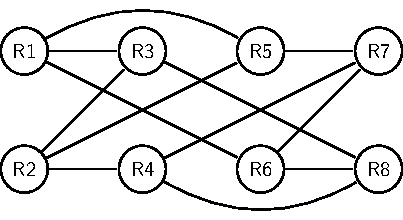
\includegraphics{Figures/extreme.pdf}
\end{center}
\caption{Extreme case for RS-B3}
\label{fig:extreme}
\end{figure}

\section{Number of Duplicates Generated}
\textbf{Claim 1}: The number of duplicates generated by \textbf{RS-B3} during the exploration of a class that combines k relations, on a completely connected graph is: $O(3^l2^r)$ \\
\textbf{Proof}: In a fully explored class that combines n relations the number of join operators is $A(n) = 2^n - 2$. Consider a class that combines $k$ relations. Using an initial element $[L]\bowtie[R]$ with $l$ the number of relations in $[L]$ and $k-l$ the number of relations in R, the transformation rules generate the following elements. Rule $R_{1}$ generates mirror image of original operator. Rule $R_{2}$ combines every element of $[L]$ with $[R]$. Note the previous step enables rule $R_{3}$. Now rule $R_{3}$ combines every element of this newly generated $[R']$ with the leftover of L. Counting the number of alternatives generates :
\begin{eqnarray*}
C &=& \sum\limits_{k=1}^{l-1} {l \choose k} A(k+r) \nonumber \\ 
 &=& \sum\limits_{k=1}^{l-1} {l \choose k} (2^{k+r} - 2) \nonumber \\
 &=& 2^r (3^l - 2^l - 1) - 2 (2^l - 2) \nonumber \\
\end{eqnarray*}

Application of rule $R_{3}$ enables commutativity which generates mirror images. To count the number of duplicates generated at this step add all the newly created operator and the initial operators and subtract $A(k)$ :
\begin{eqnarray*}
	D &=& 2 + 2*C - A(k) \nonumber \\
	  &=& 2 + 2^r (3^l - 2^l - 1) - 2 (2^l - 2) - (2^k - 2) \nonumber \\
	  &=& 3^l 2^r - 2^{k+1} - 2^r - 2^{l+1} +  8 \nonumber \\
\end{eqnarray*}